\documentclass[tikz,border=6pt]{standalone}
\usepackage{amsmath}
\usetikzlibrary{positioning}
\makeatletter
\AtBeginDocument{\global\let\pgf@selectfontorig\relax}
\makeatother

\begin{document}
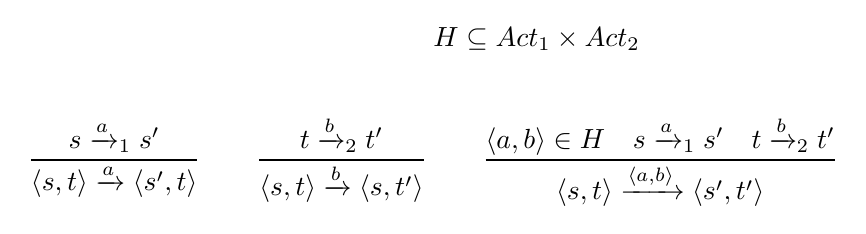
\begin{tikzpicture}
\node[inner sep=0pt, anchor=west] at (0,1.55) {$H\subseteq Act_1\times Act_2$};
\node[inner sep=0pt] {
$\displaystyle
\frac{s \xrightarrow{a}_1 s'}{\langle s,t\rangle\xrightarrow{a}\langle s',t\rangle}
\qquad
\frac{t \xrightarrow{b}_2 t'}{\langle s,t\rangle\xrightarrow{b}\langle s,t'\rangle}
\qquad
\frac{\langle a,b\rangle\in H \quad s \xrightarrow{a}_1 s' \quad t \xrightarrow{b}_2 t'}
     {\langle s,t\rangle\xrightarrow{\langle a,b\rangle}\langle s',t'\rangle}
$};
\end{tikzpicture}
\end{document}
